% Showcase Präsentation mit SimSchoolDark Theme
\documentclass{beamer}

% Theme laden
\usetheme{SimSchoolDark}

% Für Python Code Highlighting
\usepackage{listings}
\usepackage{xcolor}
\usepackage{tabu}
\usepackage{booktabs}
\usepackage{tabularx}
\usepackage[T1]{fontenc}

\definecolor{codegreen}{rgb}{0,0.6,0}
\definecolor{codegray}{rgb}{0.45,0.45,0.45}
\definecolor{codepurple}{rgb}{0.58,0,0.82}
\definecolor{backcolour}{rgb}{0.96,0.96,0.96}

\lstdefinestyle{mystyle}{
	backgroundcolor=\color{backcolour},
	commentstyle=\color{codegreen}\itshape,
	keywordstyle=\color{magenta}\bfseries,
	stringstyle=\color{codepurple},
	numberstyle=\tiny\color{codegray},
	basicstyle=\ttfamily\small,  % kompakter als footnotesize, aber noch gut lesbar
	breakatwhitespace=false,
	breaklines=true,
	captionpos=b,
	keepspaces=true,
	numbers=none,                % ich empfehle in Beamer lieber keine Zeilennummern
	showspaces=false,
	showstringspaces=false,
	showtabs=false,
	tabsize=4,                   % einheitlich 4 Spaces für Tabs
	frame=single,                % optional: Rahmen um den Code
	rulecolor=\color{gray!50},   % dezente Rahmenfarbe
	aboveskip=5pt,
	belowskip=5pt,
	xleftmargin=4pt, xrightmargin=4pt,
	columns=fullflexible         % sorgt für gleichmäßige Zeichenabstände
}

\lstset{style=mystyle}

% Python Code Style
%\lstset{
%	language=Python,
%	basicstyle=\ttfamily\small,
%	keywordstyle=\color{simschooldarkest}\bfseries,
%	stringstyle=\color{simschoolmedium},
%	commentstyle=\color{simschoollight}\itshape,
%	numberstyle=\tiny\color{simschoollight},
%	numbers=left,
%	breaklines=true,
%	frame=single,
%	rulecolor=\color{simschoolmedium},
%	backgroundcolor=\color{simschoolbg!50},
%	showstringspaces=false,
%	tabsize=4
%}

% Präsentationsinfos
\title{ARM-Embedded-Path}
\subtitle{CMSIS-Basics}
\author{Pavel Pys}
\date{\today}
%\institute{}
\begin{document}
	\begin{frame}
		\maketitle
	\end{frame}
	\begin{frame}{Overview}
		\tableofcontents
	\end{frame}
\section{Introduction}
\begin{frame}{Introduction}
	{What is the target of this journey?}
	In these slides, I want to document my learning progress in handling ARM microcontrollers, in my case from the company ST-Microelectronics. Ultimately, this slide set should become a reference work. - Hanover 21.10.2025
\end{frame}
\begin{frame}{Introduction}
	{What is the ARM architecture?}
	\begin{itemize}
		\item A microprocessor architecture developed by the British computer company Acorn in 1983. Initially, ARM stood for Acorn RISC Machine, and was later changed to Advanced RISC Machines.
		\item The company does not manufacture the chips itself, but instead grants different licenses to semiconductor development companies, which then manufacture based on this architecture.
	\end{itemize}
\end{frame}
\begin{frame}{Introduction}
	{What is the ARM architecture?}
	Today, many renowned chip manufacturers build their chips on the ARM architecture.\\
	\textbf{Notable manufacturers:}
	\begin{itemize}
		\item Apple
		\item Qualcomm Inc.
		\item Samsung Electronics
		\item Huawei Technologies Co. Ltd.
		\item STMicroelectronics
		\item ...
	\end{itemize}
\end{frame}
\begin{frame}{Introduction}
	{Market share of ARM chips}
	The market share of ARM-based chips is very large, but depends on the system. In mobile phones, it was already about 98\% in 2005 (at least one ARM processor). \\
	\vspace{0.2cm}
	In data and server centers, ARM is currently growing rapidly, though its goal of reaching 50\% market share by the end of 2025 is considered ambitious by some analysts.
\end{frame}
\begin{frame}{Introduction}
	{What are the advantages of ARM?}
	The ARM architecture offers several advantages:
	\begin{itemize}
		\item ARM uses the RISC principle.
		\item ARM cores are small and can be easily combined.
		\item Low costs and licensing flexibility.
		\item Large ecosystem.
		\item High performance per watt (efficiency).
		\item Good security features.
		\item Wide range of applications.
	\end{itemize}
\end{frame} 
\section{ARM-Architecture}
\subsection{General Information}
\begin{frame}{ARM}
	{What is a Microcontroller Architecture?}
	A microcontroller architecture describes the internal structure and functionality of a microcontroller – meaning how the individual components on the chip are interconnected and how they work together.\\
	\vspace{0.2cm}
	The architecture consists of: CPU, memory, bus system, peripherals, clock source, and power supply as well as reset logic.
\end{frame}
\begin{frame}{ARM}
	{What is a Microcontroller Architecture?}
	In summary: A microcontroller architecture is the blueprint of how CPU, memory, peripherals, buses, and clock sources work together on a single chip to execute tasks efficiently.
\end{frame}
\begin{frame}{ARM}
	{RISC vs CISC}
	\begin{figure}
		\centering
		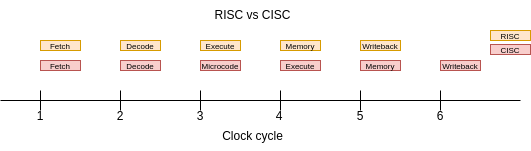
\includegraphics[width=\linewidth]{RISC_CISC_Pipe.png}
	\end{figure}
	The graphic shows the pipelines of RISC and CISC. RISC processes instructions in parallel (one new instruction per clock cycle), while CISC processes longer and more complex instructions sequentially.
\end{frame}
\begin{frame}{ARM}
	{Architecture Structure}
	Register-based design (e.g., 16-32 registers) with a pipeline architecture for parallel instruction execution.\\
	\vspace{0.2cm}
	Harvard or Von Neumann structure depending on the type.\\
	\vspace{0.2cm}
	Components:
	\begin{itemize}
		\item ALU (Arithmetic Logic Unit)
		\item Register set (R0-R15)
		\item Program Counter, Stack Pointer
		\item Interrupt Controller
		\item Bus interfaces (AHB, APB...)
	\end{itemize}
\end{frame}
\begin{frame}{ARM}
	{Architecture Structure}
	Cortex-M microcontrollers typically implement a modified Harvard architecture, where instruction and data buses are separate internally, but share a unified memory space.
\end{frame}
\subsection{ARM-Architecture}
\begin{frame}{ARM}
	{ARM - Cortex M Block-Diagram}
	\begin{figure}
		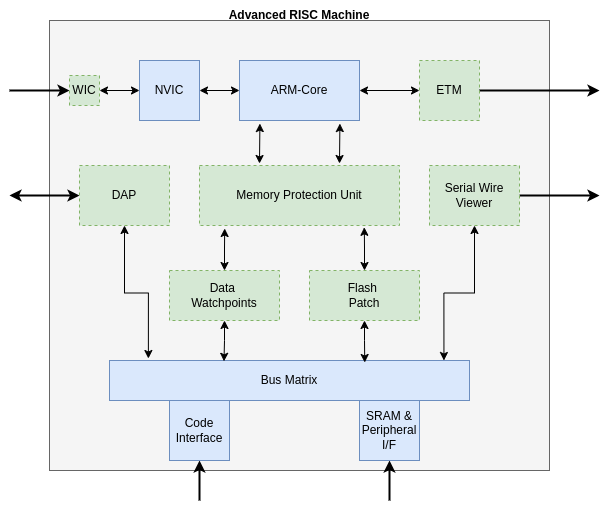
\includegraphics[width=.8\linewidth]{ARM_Block_Diagram.png}
	\end{figure}
\end{frame}
\begin{frame}{ARM}
	{WIC - Wake-up Interrupt Controller}
	In deep sleep (core clock and NVIC logic powered down), the WIC acts as a shadow interrupt latch, allowing selected IRQs to wake the system.\\
	\vspace{0.2cm}
	Control of WIC behavior through:
	\begin{itemize}
		\item NVIC->ISER (enable/disable interrupts)
		\item NVIC priorities and BASEPRI/PRIMASK (only unmasked and sufficiently prioritized IRQs can wake the system)
		\item Sleep depth via SCB->SCR.SLEEPDEEP (Deep Sleep vs. normal Sleep)
		\item WFI/WFE (how you enter sleep)
		\item Peripheral wake sources (EXTI edge, RTC alarm, USART-RX, I2C address match, etc.)
	\end{itemize}
	NVIC is tightly coupled to the Cortex-M core through the System Control Block (SCB), forming the Exception Model
\end{frame}
\begin{frame}{ARM}
	{NVIC - Nested Vector Interrupt Controller}
	The Nested Vector Interrupt Controller (NVIC) is the hardware block in the ARM Cortex-M core that:
	\begin{itemize}
		\item Accepts, prioritizes, nests, and forwards interrupts (IRQs) to the CPU,
		\item Can mask, enable, set/clear pending interrupts,
		\item Integrates exception handling (Reset, NMI, HardFault, SysTick, etc.) using the same mechanisms.
	\end{itemize}
	It is directly integrated into the core, not in the periphery, and coupled with the System Control Block (SCB).
\end{frame}
\begin{frame}{ARM}
	{ARM Core}
	The ARM core is the actual processing core (CPU core) in the microcontroller - meaning the logical unit that executes code, performs arithmetic operations, processes interrupts, and communicates with memory and peripherals via buses.\\
	\vspace{0.2cm}
	In this case (STM32F103), this is an ARM Cortex-M3, based on the ARMv7-M architecture.\\
	This means:
	\begin{itemize}
		\item 32-bit RISC processor
		\item Harvard architecture (separate buses for code and data)
		\item Pipeline design
		\item Thumb-2 instruction set (compact mix of 16- and 32-bit instructions)
	\end{itemize}
\end{frame}
\begin{frame}{ARM}
	{ARM Core: Architectural Features}
	Harvard Architecture:\\
	Separate buses for code (I-Bus) and data (D-Bus) → enables parallel reading of instructions and data\\
	\vspace{0.2cm}
	Thumb-2 Instruction Set:\\
	Mix of 16- and 32-bit instructions → compact code with full functionality\\
	\vspace{0.2cm}
	NVIC Integration:\\
	Interrupt handling directly in the core → no external interrupt controllers needed\\
	\vspace{0.2cm}
	Sleep and Deep Sleep Modes:\\
	Power saving functions via WFI/WFE instructions
\end{frame}
\begin{frame}{ARM}
	{ARM Core: Architectural Features}
	Harvard Concept in Action:
	\begin{itemize}
		\item Instructions are fetched via the I-Bus from Flash memory
		\item Data (variables, peripheral registers) via the D-Bus
		\item System and debug accesses (DMA, DAP, Trace) via the System bus
	\end{itemize}
	This allows the Cortex-M3 to simultaneously read an instruction and access data.
\end{frame}
\begin{frame}{ARM}
	{ARM Core: Conclusion}
	The ARM Cortex-M3 core is a 32-bit RISC processor with:
	\begin{itemize}
		\item Efficient pipeline design,
		\item Integrated interrupt controller,
		\item Memory protection (MPU),
		\item Integrated debug/trace architecture (CoreSight),
		\item And ideal for deterministic real-time and embedded applications (e.g., in your STM32F103).
	\end{itemize}
	It is the heart of the microcontroller - all other components (Flash, SRAM, Timer, UART, etc.) are built around it as peripherals.
\end{frame}
\begin{frame}{ARM}
	{DAP - Debug Access Port}
	The DAP (Debug Access Port) is the interface between your debugger (e.g., ST-Link, J-Link) and the internal debug and trace units of your ARM core.\\
	\vspace{0.2cm}
	The DAP acts as the "debug router" between the external world and the CoreSight internals.\\
	\vspace{0.2cm}
	The DAP consists of an AP (Access Port) and DP (Debug Port) interface – e.g. SW-DP for SWD or JTAG-DP for JTAG.
\end{frame}
\begin{frame}{ARM}
	{MPU - Memory Protection Unit}
	The MPU (Memory Protection Unit) is a hardware unit in the ARM core that divides memory into regions and monitors access rights (read/write/execute) for each region.\\
	\vspace{0.2cm}
	It prevents your code from accidentally writing to "forbidden" areas or executing from unauthorized memory.\\
	\vspace{0.2cm}
	It is thus a mini memory protection system, similar to an MMU (Memory Management Unit) in a PC - but simpler and without virtual addresses.
\end{frame}
% Slide 1: Serial Wire Viewer (SWV) Overview
\begin{frame}{ARM}
	{Serial Wire Viewer (SWV)}
	The Serial Wire Viewer is a real-time trace technology that allows debugging output with minimal overhead.\\
	\vspace{0.2cm}
	\textbf{Key Features:}
	\begin{itemize}
		\item Real-time data transmission over SWO (Serial Wire Output) pin
		\item Low overhead monitoring during program execution
		\item Part of the CoreSight debug architecture
		\item Uses ITM (Instrumentation Trace Macrocell) with internal FIFO
	\end{itemize}
	\vspace{0.2cm}
	\textbf{Common Use Cases:}
	\begin{itemize}
		\item Printf debugging via ITM
		\item Event counters and timestamps
		\item Exception trace (HardFault, interrupts)
		\item PC sampling for profiling
	\end{itemize}
	\vspace{0.2cm}
	\textbf{Note:} If ITM FIFO is full, writes may block (polling required)
\end{frame}

% Slide 2: SWV Components and Configuration
\begin{frame}{ARM}
	{SWV - Components and Configuration}
	\textbf{Hardware Components:}
	\begin{itemize}
		\item \textbf{ITM:} Instrumentation Trace Macrocell (32 stimulus ports)
		\item \textbf{DWT:} Data Watchpoint and Trace unit (PC sampling, cycle counting)
		\item \textbf{TPIU:} Trace Port Interface Unit (formats and outputs trace data)
		\item \textbf{SWO:} Serial Wire Output pin (shares pin with JTAG TDO)
	\end{itemize}
	\vspace{0.2cm}
	\textbf{Important:} SWO only works with SWD debug mode, not parallel to JTAG!
	\vspace{0.2cm}
	\textbf{Configuration Requirements:}
	\begin{itemize}
		\item Enable trace in DEMCR register
		\item Configure SWO pin speed (must match debugger)
		\item Enable desired ITM stimulus ports
		\item Set up DWT for PC sampling or data trace if needed
	\end{itemize}
\end{frame}

% Slide 3: SWV Practical Example
\begin{frame}[fragile]{ARM}
	{SWV - Practical Printf Example}
	\textbf{ITM Printf Implementation:}
	\begin{lstlisting}[language=C, basicstyle=\ttfamily\tiny]
		#include "core_cm3.h"
		
		int _write(int file, char *ptr, int len) {
			for (int i = 0; i < len; i++) {
				// Poll: 0 = FIFO full/port disabled
				//       1 = at least one word fits
				while ((ITM->PORT[0].u32 & 1) == 0);
				
				// Send character
				ITM->PORT[0].u8 = *ptr++;
			}
			return len;
		}
		
		int main(void) {
			// Enable TRCENA in DEMCR
			CoreDebug->DEMCR |= CoreDebug_DEMCR_TRCENA_Msk;
			
			// Enable ITM stimulus port 0
			ITM->TER |= (1 << 0);
			
			printf("Hello from SWV!\n");
			while(1);
		}
	\end{lstlisting}
\end{frame}

% Slide 4: Data Watchpoints Overview
\begin{frame}{ARM}
	{Data Watchpoints (DWT)}
	The Data Watchpoint and Trace (DWT) unit provides hardware-based memory access monitoring and performance profiling.\\
	\smallskip
	\textbf{Core Capabilities:}
	\begin{itemize}
		\item Comparators for watchpoints (implementation dependent)
		\item Number available in DWT\_CTRL.NUMCOMP (typically 4 on Cortex-M3)
		\item Monitor read, write, or read/write access to memory addresses
		\item Generate debug events or trigger trace without stopping CPU
		\item Cycle counter (CYCCNT) for precise timing measurements
	\end{itemize}
	\smallskip
	\textbf{Use Cases:}
	\begin{itemize}
		\item Detect when a variable is modified (data breakpoint)
		\item Profile code execution time
		\item Trace memory access patterns
		\item Detect buffer overruns or stack corruption
	\end{itemize}
\end{frame}

% Slide 5: DWT Configuration and Registers
\begin{frame}{ARM}
	{Data Watchpoints - Configuration}
	\textbf{Key DWT Registers (per comparator):}
	\begin{itemize}
		\item \textbf{DWT\_COMPn:} Address to watch
		\item \textbf{DWT\_MASKn:} Address range (0 = exact match, 1-31 = range size)
		\item \textbf{DWT\_FUNCTIONn:} Function control (read/write, size, action)
	\end{itemize}
	\vspace{0.2cm}
	\textbf{FUNCTION Register Options (see ARMv7-M TRM):}
	\begin{itemize}
		\item FUNCTION[3:0] = Match mode (data read/write, PC match, etc.)
		\item DATAVSIZE[1:0] = Data size (byte, halfword, word)
		\item Action: Generate debug event or emit trace packet
	\end{itemize}
	\vspace{0.2cm}
	\textbf{Additional DWT Features:}
	\begin{itemize}
		\item \textbf{DWT\_CYCCNT:} Cycle counter (free-running 32-bit)
		\item \textbf{DWT\_CTRL:} Enable cycle counter, read NUMCOMP
	\end{itemize}
\end{frame}

% Slide 6: DWT Practical Example
\begin{frame}[fragile]{ARM}
	{Data Watchpoints - Practical Example}
	\textbf{Watch a variable for writes:}
	\begin{lstlisting}[language=C, basicstyle=\ttfamily\tiny]
		volatile uint32_t critical_var = 0;
		
		void setup_watchpoint(void) {
			// Enable TRCENA
			CoreDebug->DEMCR |= CoreDebug_DEMCR_TRCENA_Msk;
			
			// Comparator 0: Watch critical_var
			DWT->COMP0 = (uint32_t)&critical_var;
			DWT->MASK0 = 0;  // Exact match
			
			// FUNCTION: Use CMSIS symbols or see ARMv7-M TRM Table B3-11
			// Example: Data write match (exact bits depend on implementation)
			// Refer to: interrupt.memfault.com/blog/cortex-m-watchpoints
			DWT->FUNCTION0 = (1 << 4) |  // DATAVMATCH
			(1 << 0);    // FUNCTION bits (consult TRM)
		}
		
		int main(void) {
			setup_watchpoint();
			
			critical_var = 42;  // Triggers watchpoint!
			while(1);
		}
	\end{lstlisting}
\end{frame}

% Slide 7: Flash Patch and Breakpoint (FPB) Overview
\begin{frame}{ARM}
	{Flash Patch and Breakpoint Unit (FPB)}
	The FPB allows setting breakpoints in code memory and optionally patching code execution to RAM.\\
	\vspace{0.2cm}
	\textbf{Two Main Functions:}
	\begin{itemize}
		\item \textbf{Breakpoints:} Instruction comparators (implementation dependent)
		\item \textbf{Code Patching:} Remap to RAM (if RMPSPT flag supported)
	\end{itemize}
	\vspace{0.2cm}
	\textbf{Implementation Dependent (read FP\_CTRL):}
	\begin{itemize}
		\item NUM\_CODE: Instruction comparators (typically 6 on Cortex-M3)
		\item NUM\_LIT: Literal comparators (typically 2)
		\item RMPSPT: Remap support flag (not always present)
	\end{itemize}
	\vspace{0.2cm}
	\textbf{Note:} FPB is a debug feature, not intended for field updates. Code region base depends on MCU memory map (e.g., STM32: 0x0800\_0000).
\end{frame}

% Slide 8: FPB Configuration and Registers
\begin{frame}{ARM}
	{Flash Patch - Configuration}
	\textbf{Key FPB Registers:}
	\begin{itemize}
		\item \textbf{FP\_CTRL:} Enable FPB, read NUM\_CODE/NUM\_LIT/RMPSPT
		\item \textbf{FP\_COMPn:} Comparator n configuration
		\item \textbf{FP\_REMAP:} Base address of replacement code in RAM
	\end{itemize}
	\vspace{0.2cm}
	\textbf{Comparator Configuration (FP\_COMPn):}
	\begin{itemize}
		\item Bit [0]: ENABLE (1 = active)
		\item Bits [1:0]: REPLACE field (2-bit, see ARMv7-M TRM)
		\begin{itemize}
			\item 00 = Remap to RAM (if RMPSPT supported)
			\item 01/10/11 = Breakpoint on instruction/halfword
		\end{itemize}
		\item Bits [31:2]: Code address bits [31:2] (word-aligned)
	\end{itemize}
	\vspace{0.2cm}
	\textbf{References:}
	\begin{itemize}
		\item ARMv7-M Architecture Reference Manual (Section C1.11)
		\item Doulos Application Note on FPB
	\end{itemize}
\end{frame}

% Slide 9: FPB Practical Example
\begin{frame}[fragile]{ARM}
	{Flash Patch - Practical Example}
	\textbf{Patch a buggy function in Flash:}
	\begin{lstlisting}[language=C, basicstyle=\ttfamily\tiny]
		// Buggy function in Flash
		void buggy_function(void) {
			// Contains a bug
		}
		
		// Fixed version in RAM
		__attribute__((section(".data")))
		void fixed_function(void) {
			// Corrected implementation
		}
		
		void setup_flash_patch(void) {
			// Check if remap is supported
			if (!(FP->CTRL & FP_CTRL_KEY_Msk)) return;
			
			// Enable FPB
			FP->CTRL |= FP_CTRL_ENABLE_Msk | FP_CTRL_KEY_Msk;
			
			// Set remap base (SRAM start, shifted right by 5)
			FP->REMAP = 0x20000000 >> 5;
			
			// Comparator 0: Remap buggy_function to fixed_function
			// REPLACE = b00 for remap, ENABLE = 1
			uint32_t flash_addr = (uint32_t)buggy_function;
			FP->COMP[0] = (flash_addr & ~0x3u) | 1u;  // ENABLE=1, REPLACE=00
		}
	\end{lstlisting}
\end{frame}

% Slide 10: Debug Features Comparison
\begin{frame}{ARM}
	{Debug Features - Quick Comparison}
	\begin{center}
		\small
		\begin{tabular}{|l|l|l|}
			\hline
			\textbf{Feature} & \textbf{Purpose} & \textbf{Overhead} \\ \hline
			SWV/ITM & Printf, trace output & Low (FIFO may block) \\ \hline
			DWT & Data watchpoints, profiling & Minimal \\ \hline
			FPB & Breakpoints, code patching & Debug-only \\ \hline
		\end{tabular}
	\end{center}
	
	\vspace{0.2cm}
	\textbf{Resource Limits (implementation dependent):}
	\begin{itemize}
		\item ITM: 32 stimulus ports
		\item DWT: Read DWT\_CTRL.NUMCOMP (typically 4)
		\item FPB: Read FP\_CTRL.NUM\_CODE/NUM\_LIT (typically 6+2)
	\end{itemize}
	
	\vspace{0.2cm}
	\textbf{Common Debugger Support:}
	\begin{itemize}
		\item J-Link: Full support for all features
		\item ST-Link: SWV supported, limited FPB
		\item OpenOCD: Basic SWV, DWT support
	\end{itemize}
\end{frame}
\subsection{CMSIS vs HAL}
\begin{frame}[fragile]
	\frametitle{CMSIS vs HAL}
	\framesubtitle{CMSIS (Cortex Microcontroller Software Interface Standard)}
	\begin{lstlisting}[language=C]
// Direct register access
RCC->APB2ENR |= RCC_APB2ENR_IOPCEN;  // Enable clock
GPIOC->BSRR = GPIO_BSRR_BR13;        // Set pin to LOW
	\end{lstlisting}
	\begin{itemize}
		\item Vendor: ARM (Cortex-M standard)
		\item Abstraction level: Low (register-level via CMSIS-Device headers)
		\item What is it?: Standardized core intrinsics + device header mapping (names/addresses)
	\end{itemize}
\end{frame}
\begin{frame}[fragile]
	\frametitle{CMSIS vs HAL}
	\framesubtitle{HAL (Hardware Abstraction Layer)}
	\begin{lstlisting}[language=C]
// Function calls
__HAL_RCC_GPIOC_CLK_ENABLE();           // Enable clock
HAL_GPIO_WritePin(GPIOC, GPIO_PIN_13, GPIO_PIN_RESET);  // Set pin to LOW
	\end{lstlisting}
	\begin{itemize}
		\item Vendor: STMicroelectronics (only for STM32)
		\item Abstraction level: High (hides registers)
		\item What is it?: Convenient function library
	\end{itemize}
\end{frame}
\begin{frame}[fragile]
	\frametitle{CMSIS vs HAL}
	\framesubtitle{Turning LED on - Both approaches:}
	CMSIS:
	\begin{lstlisting}[language=C]
RCC->APB2ENR |= RCC_APB2ENR_IOPCEN;
GPIOC->CRH &= ~(GPIO_CRH_CNF13 | GPIO_CRH_MODE13);
GPIOC->CRH |= GPIO_CRH_MODE13_1;
GPIOC->BSRR = GPIO_BSRR_BR13;
	\end{lstlisting}
	\begin{itemize}
		\item 4 lines of code
		\item You need to understand registers
		\item Fast (direct)
	\end{itemize}
\end{frame}
\begin{frame}{CMSIS vs HAL}
	{Turning LED on - Both approaches:}
	HAL:
	\begin{itemize}
		\item 7+ lines of code
		\item Readable and self-explanatory
		\item Slower (many function calls)
	\end{itemize}
	\vspace{0.2cm}
	HAL typically requires more lines of code due to function calls and initializations.
\end{frame}
\begin{frame}{CMSIS vs HAL}
	\small
	\begin{tabularx}{\linewidth}{@{} l >{\raggedright\arraybackslash}X >{\raggedright\arraybackslash}X @{}}
		\toprule
		\textbf{Aspect} & \textbf{CMSIS / Register} & \textbf{HAL (STM32)} \\
		\midrule
		Performance & typically $3$--$10\times$ faster\textsuperscript{*} & slower (wrapper calls) \\
		Code size (blink) & $\sim$3--6 KB & $\sim$15--25 KB \\
		Learning curve & steeper & flatter \\
		Readability & terse / technical & very readable \\
		Portability & vendor-agnostic concepts; device headers per family & portable within STM32 family \\
		Debugging & transparent (no hidden layers) & black-boxy at times \\
		Control & 100\% & limited by API \\
		\bottomrule
	\end{tabularx}
	
	\medskip
	{\footnotesize\textsuperscript{*}\,Can be much more in tight loops/ISRs, depends on inlining and wait states.}
\end{frame}

\begin{frame}[fragile]
	\frametitle{CMSIS vs HAL}
	\framesubtitle{Why should you learn CMSIS?}
	Understand how hardware REALLY works.
	\begin{lstlisting}[language=C]
// HAL hides the magic
HAL_GPIO_WritePin(GPIOC, GPIO_PIN_13, GPIO_PIN_RESET);
		
// CMSIS shows you the reality
GPIOC->BSRR = GPIO_BSRR_BR13;  // Set bit 29 in register 0x4001100C
	\end{lstlisting}
	With CMSIS you understand that you're setting a specific bit in a hardware register. \textbf{With HAL you're just calling a function.}
\end{frame}
\begin{frame}[fragile]
	\frametitle{CMSIS vs HAL}
	\framesubtitle{Performance in Time-Critical Applications}
	\begin{lstlisting}[language=C]
// HAL: ~50-100 CPU cycles
HAL_GPIO_WritePin(GPIOC, GPIO_PIN_13, GPIO_PIN_SET);
		
// CMSIS: ~2-3 CPU cycles
GPIOC->BSRR = GPIO_BSRR_BS13;
	\end{lstlisting}
	At 72 MHz: HAL takes ~1.4 µs, CMSIS only ~0.04 µs - 35x faster!\\
	\vspace{0.2cm}
	Important for: Fast PWM, Bit-banging (WS2812 LEDs, OneWire), Interrupt Service Routines and real-time protocols\\
	\vspace{0.2cm}
	\footnotesize{Exact cycle counts depend on compiler optimization, inlining and bus wait states.
		Rule of thumb: CMSIS/register-level calls are typically an order of magnitude faster than HAL wrappers.}
	
\end{frame}
\begin{frame}[fragile]
	\frametitle{CMSIS vs HAL}
	\framesubtitle{Smaller Code = More Space for Your Program}
	\begin{lstlisting}[language=C]
STM32F103C6: 32 KB Flash
		
HAL project:    HAL library ≈ 15–25 KB → Leaves ~7–17 KB for your code
CMSIS project:  CMSIS only ≈ 3–6 KB   → Leaves ~26–29 KB for your code
	\end{lstlisting}
	\vspace{0.2cm}
	\footnotesize{Note: The exact size depends on which HAL modules are linked. 
		Even small HAL-based projects often use significantly more Flash due to 
		abstraction layers and initialization code.}
\end{frame}
\begin{frame}[fragile]
	\frametitle{CMSIS vs HAL}
	\framesubtitle{Understanding Other MCUs}
	When you switch to other manufacturers (ESP32, Nordic nRF, Raspberry Pi Pico),	there is no STM32 HAL. Each vendor provides its own SDK (e.g., ESP-IDF, nRF5).
	But the register-level principle remains the same.
	\begin{lstlisting}[language=C]
// STM32 (CMSIS)
GPIOC->BSRR = GPIO_BSRR_BS13;
// ESP32 (IDF)
GPIO.out_w1ts = (1 << 13);
// nRF52 (Nordic)
NRF_GPIO->OUTSET = (1 << 13);
	\end{lstlisting}
\end{frame}
\begin{frame}{CMSIS vs HAL}
	{Jobs and Industry}
	In industry among professional embedded developers:\\
	\vspace{0.2cm}
	HAL: ~20\% (prototyping, quick projects)\\
	CMSIS/Register-Level: ~80\% (production, performance)\\
	\vspace{0.2cm}
	Why? Because:
	\begin{itemize}
		\item Firmware must be small (cheaper MCUs)
		\item Firmware must be fast (real-time requirements)
		\item Developers must understand hardware (troubleshooting)
	\end{itemize}
\end{frame}
\section{Practice}
\subsection{Blink-Test:Mixed}
\begin{frame}{Practice}
	{Blink Test}
	Just as the "Hello World" project is commonly used in pure software programming, here a Blink project is described. This project makes an arbitrary LED blink using an ARM microcontroller. In my case, a \textbf{STM32F103C6T6A}.
	\begin{figure}
		\centering
		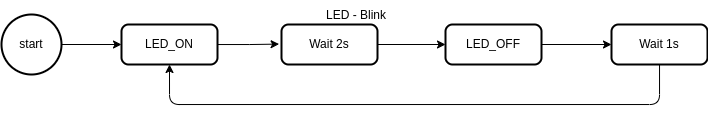
\includegraphics[width=\linewidth]{LED_Blink_Flow.png}
	\end{figure}
\end{frame}
\begin{frame}{Practice}
	{Blink Test}
	The program flow is simple: The LED is turned on, this state is maintained for 2 seconds, then the LED is turned off and the processor waits for 1 second before the LED turns on again. This sequence is then executed continuously through a loop.\\ 
	\vspace{0.2cm}
	In my case, the LED is controlled via pin PC13. Flashing and debugging is done using an ST-Link, therefore in CubeIDE the debug parameter must be set to Serial Wire.
\end{frame}
\begin{frame}{Practice}
	{CubeIDE Configuration}
	\begin{figure}
		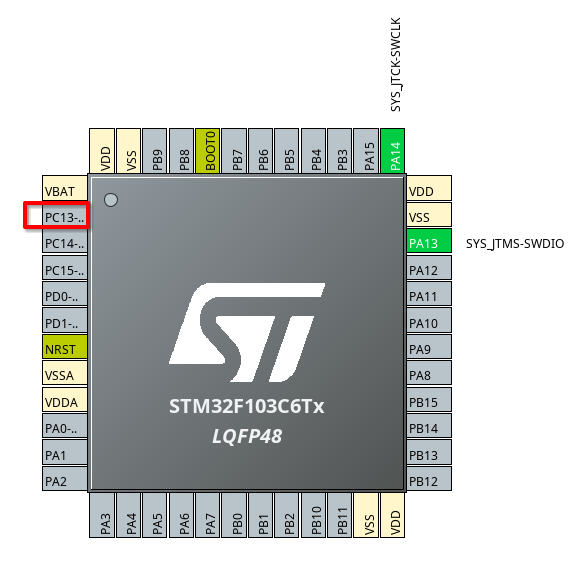
\includegraphics[width=.6\linewidth]{Blink_001.png}
	\end{figure}
	The pin \textbf{PC13} is configured directly in the code.
\end{frame}
\begin{frame}{Practice}
	{CubeIDE Configuration}
	\begin{figure}
		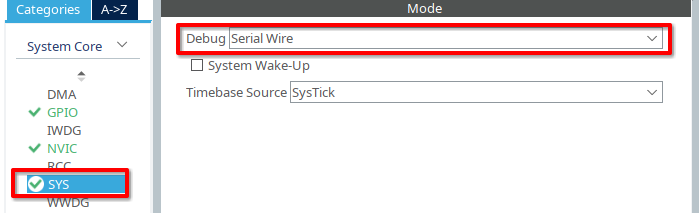
\includegraphics[width=\linewidth]{Blink_002.png}
	\end{figure}
\end{frame}
\begin{frame}{Practice}
	{Useing HAL}
	Although HAL is not the main topic here, it’s interesting to see how the same project looks using the HAL library.
	
\end{frame}
\begin{frame}[fragile]
	\frametitle{Implementation with HAL}
	\begin{lstlisting}[language=C]
int main(void)
	{
		HAL_Init();
		SystemClock_Config();
		MX_GPIO_Init();
		while (1)
		{
			....
		}
	}
	\end{lstlisting}
	The GPIO configuration is implemented directly by the HAL library, whereas in CMSIS you have to configure the registers yourself.
\end{frame}
\begin{frame}[fragile]
	\frametitle{Implementation with HAL}
	\begin{lstlisting}[language=C]
while (1)
	{
		// LED ON for 2 seconds (active-low: GPIO_PIN_RESET)
		HAL_GPIO_WritePin(GPIOC, GPIO_PIN_13, GPIO_PIN_RESET);
		HAL_Delay(2000);
			
		// LED OFF for 1 second (active-high: GPIO_PIN_SET)
		HAL_GPIO_WritePin(GPIOC, GPIO_PIN_13, GPIO_PIN_SET);
		HAL_Delay(1000);
	}
	\end{lstlisting}
	Delay and WritePin functions are also provided by the HAL library, the code closely resembles Arduino code.
\end{frame}
\begin{frame}{Practice}
	{Functional Architecture and Logic}
	For the LED to blink (toggle), the MCU must know exactly when it should be ON, how long it should be ON, and when the LED must be turned OFF. For this, a delay function implemented with the SysTick\_Handler is used.
	\begin{figure}
		\centering
		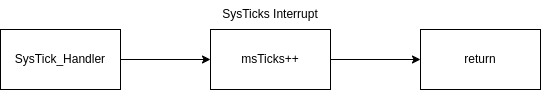
\includegraphics[width=\linewidth]{Blink_003.png}
	\end{figure}
\end{frame}
\begin{frame}{Practice}
	{Functional Architecture and Logic}
	\textbf{SysTick\_Handler:} The SysTick is a timer in the processor that triggers an interrupt at regular intervals (here every millisecond). It's like an alarm clock that rings every millisecond. When the alarm rings, the \textbf{SysTick\_Handler} function is called. This function does only one thing: it increments the counter \textbf{msTicks} by 1.\\
	\vspace{0.2cm}
	\textbf{Interrupt:} Imagine you are a teacher grading exams (that's your main program). Suddenly the telephone rings (that's the interrupt). You interrupt the grading, answer the phone and talk to the caller (that's the interrupt handler). When the call is finished, you return to grading and continue exactly where you left off.
\end{frame}
\begin{frame}{Practice}
	{Functional Architecture and Logic}
	\begin{figure}
		\centering
		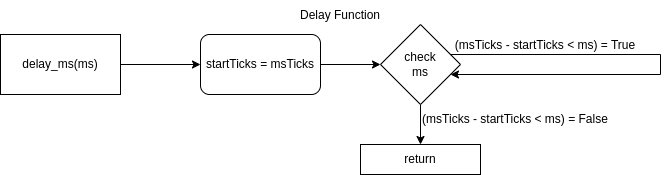
\includegraphics[width=\linewidth]{Blink_004.png}
	\end{figure}
	The system utilizes a delay function that waits for milliseconds. It is based on a global counter \textbf{msTicks} that is incremented every millisecond by the SysTick interrupt.
	
	The function stores the current value of \textbf{msTicks} at the beginning (\textbf{startTicks}). It then waits in a loop until the difference between the current \textbf{msTicks} and \textbf{startTicks} becomes greater than or equal to the desired \textbf{ms} value.
\end{frame}
\begin{frame}[fragile]
	\frametitle{Practice}
	\framesubtitle{Functional Architecture and Logic}
	\begin{lstlisting}[language=C]
void delay_ms(uint32_t ms){
	uint32_t startTicks = msTicks;
	while ((msTicks - startTicks) < ms);
}
	\end{lstlisting}
	The msTicks counter overflows after approximately 49 days from 4,294,967,295 to 0, but the calculation (msTicks - startTicks) still functions correctly because subtraction with unsigned integers always produces the correct result.\\
	\vspace{0.2cm}
	This approach utilizes the hardware timer (not "estimated" waiting), ensuring that 1000ms are exactly 1000ms.
\end{frame}
\begin{frame}{Practice}
	{Functional Architecture and Logic}
	Why uint32\_t:\\
	\textbf{System independence}: If one uses int, the compiler might allocate different memory sizes (e.g., 2 bytes on a 16-bit system vs. 4 bytes on a 32-bit system). uint32\_t ensures that the data type is always exactly 32 bits, regardless of the architecture.\\
	\vspace{0.2cm}
	\textbf{Hardware registers}: When programming microcontrollers such as an STM32, one often needs to work with hardware registers that have a fixed bit width (e.g., 32 bits). uint32\_t fits perfectly and facilitates bit manipulation.\\
\end{frame}
\begin{frame}[fragile]
	\frametitle{Practice}
	\framesubtitle{Functional Architecture and Logic}
	This example utilizes the internal clock source.
	\begin{lstlisting}[language=C]
void SystemClock_Config(void){
	RCC_OscInitTypeDef RCC_OscInitStruct = {0};
	RCC_ClkInitTypeDef RCC_ClkInitStruct = {0};
			
	// HSI as oscillator
	RCC_OscInitStruct.OscillatorType = RCC_OSCILLATORTYPE_HSI;
	RCC_OscInitStruct.HSIState = RCC_HSI_ON;
	// No PLL used
	RCC_OscInitStruct.PLL.PLLState = RCC_PLL_NONE;
}
	\end{lstlisting}
\end{frame}
\begin{frame}[fragile]
	\frametitle{Practice}
	\framesubtitle{Functional Architecture and Logic}
	\begin{itemize}
		\item Configures the internal 8MHz oscillator (HSI)
		\item No clock division for buses
		\item Simplest clock configuration
	\end{itemize}
	\begin{lstlisting}[language=C]
SysTick_Config(SystemCoreClock / 1000);
	\end{lstlisting}
	Configures the SysTick timer for an interrupt every 1ms.\\
	SystemCoreClock / 1000 divides the CPU clock frequency by 1000 for 1ms intervals. During each interrupt, msTicks is incremented.
\end{frame}
\begin{frame}{Practice}
	{Functional Architecture and Logic}
	What happens if the clock configuration is not performed or is performed incorrectly?\\
	\textbf{SystemClock\_Config()}:\\
	This function configures the system clock. Without it, the microcontroller runs with the default clock (e.g., internal HSI oscillator), but potentially not at the expected frequency.\\
	\vspace{0.2cm}
	Specifically, it enables the HSI (Internal High-Speed Clock) and sets the clock frequency for the CPU and peripherals.\\
	\vspace{0.2cm}
	Without clock configuration, the clock might be too slow or might not run at all, causing the microcontroller to malfunction.
\end{frame}
\begin{frame}{Practice}
	{Functional Architecture and Logic}
	\textbf{SysTick\_Config()}:\\
	This function configures the SysTick timer, which is required for the delay\_ms function. Without it, msTicks is not incremented, and the delay function would wait indefinitely.\\
	\vspace{0.2cm}
	\textbf{GPIO\_LED\_Init()}:\\
	This function activates the clock for GPIOC via RCC->APB2ENR |= RCC\_APB2ENR\_IOPCEN.   
	For the GPIOC clock to be activated, the RCC (Reset and Clock Control) module itself must be properly clocked. This is ensured by SystemClock\_Config().  
	Without the system clock, setting the RCC\_APB2ENR\_IOPCEN bit might have no effect because the RCC module is not operational.
\end{frame}
\begin{frame}{Practice}
	{Functional Architecture and Logic}
	\begin{block}{Summary}
		Without clock configuration, the microcontroller remains in a reset state or operates with an unconfigured clock, resulting in no peripherals (including GPIO) functioning. The GPIO initialization assumes that the system clock has already been configured.
	\end{block}
\end{frame}
\begin{frame}[fragile]
	\frametitle{Practice}
	\framesubtitle{Functional Architecture and Logic}
	\begin{lstlisting}[language=C]
void GPIO_LED_Init(void){
// Enable clock
RCC->APB2ENR |= RCC_APB2ENR_IOPCEN;
			
// Configure pin
GPIOC->CRH &= ~(GPIO_CRH_CNF13 | GPIO_CRH_MODE13);
GPIOC->CRH |= GPIO_CRH_MODE13_1;
			
// Turn off LED initially
GPIOC->BSRR = GPIO_BSRR_BS13;
}
	\end{lstlisting}
\end{frame}
\begin{frame}{Practice}{Functional Architecture and Logic}
	\textbf{Enable GPIOC clock (RCC\_APB2ENR)}
	\medskip
	
	\texttt{RCC->APB2ENR |= RCC\_APB2ENR\_IOPCEN}
	
	\medskip
	Enables the peripheral clock for \textbf{GPIO port C}. The bit lives in the
	STM32 reference manual under \emph{RCC\_APB2ENR — APB2 peripheral clock enable register}
	(field \textbf{IOPCEN}).
	
	\medskip
	The compound operator \texttt{|=} performs a \emph{read–modify–write}:
	\begin{enumerate}
		\item Read the current value of \texttt{RCC->APB2ENR}.
		\item OR it with the mask \texttt{RCC\_APB2ENR\_IOPCEN}.
		\item Write the result back to \texttt{RCC->APB2ENR}.
	\end{enumerate}
	
	\smallskip
	\textit{Note:} \texttt{RCC\_APB2ENR\_IOPCEN} equals \texttt{(1u << 4)} (i.e., only bit~4 set).
\end{frame}
\begin{frame}{Practice}{Functional Architecture and Logic}
	\textbf{Why not use \texttt{=}?}
	\medskip
	
	The advantage of \texttt{|=} is that it \textbf{sets exactly one bit} and \textbf{leaves all other bits untouched}.
	
	\medskip
	If you wrote \texttt{RCC->APB2ENR = RCC\_APB2ENR\_IOPCEN} you would:
	\begin{itemize}
		\item enable GPIOC,
		\item \textbf{but clear every other bit} in the register — disabling any APB2 peripheral that was previously enabled (AFIO, GPIOA/B, ADC1, \dots).
	\end{itemize}
	
	\medskip
	\textbf{Conclusion:}
	\begin{itemize}
		\item use \texttt{|=} to \textbf{set} bits,
		\item use \texttt{\&= \textasciitilde mask} to \textbf{clear} bits (e.g., \texttt{RCC->APB2ENR \&= \textasciitilde RCC\_APB2ENR\_IOPCEN;}).
	\end{itemize}
\end{frame}
\begin{frame}{Practice}{Functional Architecture and Logic}
	\textbf{About the macro}
	\medskip
	
	\texttt{RCC\_APB2ENR\_IOPCEN} is a descriptive macro provided by STMicroelectronics in the device header.
	It expands to the bit mask \texttt{(1u << 4)}, i.e., only bit~4 is set.
	
	\medskip
	Therefore the following are \textbf{equivalent}:
	\begin{itemize}
		\item \texttt{RCC->APB2ENR |= (1u << 4);}
		\item \texttt{RCC->APB2ENR |= RCC\_APB2ENR\_IOPCEN;}
	\end{itemize}
	
	Using the named macro is \textbf{clearer} and often more \textbf{portable} across STM32 families,
	where bit positions may differ.
	
	\medskip
	\textit{Good practice:} enable the port clock \emph{before} writing any GPIO registers for that port.
\end{frame}
\begin{frame}[fragile]{Practice}{Bit-Masking: Clear Bits Operation}
	\textbf{Why \&= \textasciitilde( ... )?}\\
	This is a "clear bits" step:
	\begin{itemize}
		\item \texttt{GPIO\_CRH\_CNF13 | GPIO\_CRH\_MODE13} creates a mask covering all 4 bits of Pin 13 (CNF + MODE).
		\item \texttt{\textasciitilde(...)} inverts the mask $\rightarrow$ ones everywhere, except these 4 bits (there 0).
		\item \texttt{\&=} with this inverted mask sets exactly these 4 bits to 0, leaving all other bits unchanged.
	\end{itemize}
	\textbf{Purpose:} Clear the 4 configuration bits of PC13 so no old state remains.
	\medskip
	
	\texttt{GPIOC->CRH \&= \textasciitilde(0xFu << 20);}
\end{frame}
\begin{frame}{Practice}{Pin Configuration: CNF and MODE Bits}
	\textbf{Each GPIO pin uses 4 bits: [CNF1 CNF0 MODE1 MODE0]}
	\medskip
	
	\textbf{MODE[1:0] (outputs speed / input select):}
	\begin{itemize}
		\item 00 = Input mode
		\item 01 = Output 10\,MHz
		\item 10 = Output 2\,MHz
		\item 11 = Output 50\,MHz
	\end{itemize}
	
	\textbf{CNF[1:0] (depends on MODE):}
	\begin{itemize}
		\item \textbf{If MODE=00 (input):} 00=Analog,\; 01=Floating,\; 10=Pull-up/Down,\; 11=Reserved
		\item \textbf{If MODE$\neq$00 (output):} 00=General-Purpose Push-Pull,\; 01=General-Purpose Open-Drain,\\
		10=Alternate-Function Push-Pull,\; 11=Alternate-Function Open-Drain
	\end{itemize}
\end{frame}
\begin{frame}{Practice}{GPIO Reset State \& Safe Pattern}
	\textbf{After reset:}
	\begin{itemize}
		\item All GPIOs: \texttt{MODE=00} (Input), \texttt{CNF=01} (Floating input)
		\item Debug pins (JTAG/SWD) are mapped to debug by default (free via \texttt{AFIO\_MAPR})
	\end{itemize}
	
	\textbf{Why this matters:}
	\begin{itemize}
		\item Setting only \texttt{MODE} leaves \texttt{CNF} as-is.
		\item Example: \texttt{MODE=10} with leftover \texttt{CNF=01} $\Rightarrow$ \textbf{general-purpose open-drain output}
		(not invalid, but often unintended for LEDs; cannot actively drive HIGH without pull-up).
	\end{itemize}
	
	\textbf{Safe approach (clean-then-set):}
	\begin{itemize}
		\item \texttt{GPIOC->CRH \&= \textasciitilde(0xFu << 20);} \quad // clear CNF:MODE for PC13
		\item \texttt{GPIOC->CRH |=  (0x2u < 20);} \quad // CNF=00, MODE=10 $\Rightarrow$ Output 2\,MHz push-pull
	\end{itemize}
	
	\textbf{Key takeaway:} Always \texttt{Clock $\rightarrow$ Clear $\rightarrow$ Set}.
\end{frame}
\begin{frame}{Practice}{Setting MODE Bits – Risky Approach}
	\textbf{Make PC13 an Output @ 2\,MHz (keep CNF unchanged)}
	\medskip
	
	\texttt{GPIOC->CRH |= GPIO\_CRH\_MODE13\_1;}
	
	\medskip
	What this does:
	\begin{itemize}
		\item \texttt{GPIO\_CRH\_MODE13\_1 = 0x00200000} sets bit 21
		\item Result: \texttt{MODE13 = 10b} → Output 2\,MHz
		\item \textcolor{red}{\textbf{Problem:}} CNF bits are NOT modified!
	\end{itemize}
	
	\textbf{Why is this risky?}
	\begin{itemize}
		\item After reset: CNF=01, MODE=00
		\item After this line: CNF=01, MODE=10 → invalid config!
	\end{itemize}
	
	\textbf{Safe only if:} CNF was already set correctly before.
\end{frame}
\begin{frame}[fragile]{Practice}{Best Practice: Clean-then-Set Pattern}
	\textbf{Recommended approach (always safe):}
	\begin{lstlisting}[language=C, basicstyle=\ttfamily\small]
// Clear all 4 bits (CNF + MODE)
GPIOC->CRH &= ~(0xFu << 20);
		
// Set new configuration
GPIOC->CRH |= (0x2u << 20);
	\end{lstlisting}
	
	\textbf{What happens:}
	\begin{itemize}
		\item \texttt{0xFu << 20 = 0x00F00000} masks bits 23..20
		\item Clear these 4 bits, keep all others
		\item \texttt{0x2u << 20 = 0x00200000} sets CNF=00, MODE=10
	\end{itemize}
	
	\textbf{Calculation:} PC13 in CRH at $(13-8) \times 4 = 20$
\end{frame}
\begin{frame}[fragile]{Practice}{Complete Example: PC13 Configuration}
	\textbf{Configure PC13 as Output Push-Pull, 2\,MHz}
	
	\begin{lstlisting}[language=C, basicstyle=\ttfamily\footnotesize]
// 1. Enable GPIO Clock (CRITICAL!)
RCC->APB2ENR |= RCC_APB2ENR_IOPCEN;
		
// 2. Clear PC13 config (bits 23..20)
GPIOC->CRH &= ~(0xFu << 20);
		
// 3. Set: CNF=00, MODE=10 (2 MHz)
GPIOC->CRH |= (0x2u << 20);
	\end{lstlisting}
	
	\textbf{Three essential steps:}
	\begin{enumerate}
		\item Enable Clock – without this, writes are ignored!
		\item Clear – remove old configuration
		\item Set – apply new configuration
	\end{enumerate}
\end{frame}
\begin{frame}[fragile]{Practice}{Bit Position Calculation}
	\textbf{General Formula:}\\
	\texttt{value = ((CNF << 2) | MODE) << offset}
	
	\medskip
	\textbf{Offset Calculation:}
	\begin{itemize}
		\item \textbf{CRL (pins 0..7):} \texttt{offset = pin\_number * 4}
		\item \textbf{CRH (pins 8..15):} \texttt{offset = (pin\_number - 8) * 4}
	\end{itemize}
	
	\textbf{Examples:}
	\begin{itemize}
		\item PA3: CRL, offset = $3 \times 4 = 12$
		\item PC13: CRH, offset = $(13-8) \times 4 = 20$
		\item PB15: CRH, offset = $(15-8) \times 4 = 28$
	\end{itemize}
	
	\textbf{PA3 Output PP, 50 MHz:}\\
	\texttt{GPIOA->CRL \&= \textasciitilde(0xFu << 12);}\\
	\texttt{GPIOA->CRL |= (0x3u << 12);}
\end{frame}
\begin{frame}{Reference}{Quick Reference}
	\begin{center}
		\small
		\begin{tabular}{|c|l|l|}
			\hline
			\textbf{CNF} & \textbf{Output (MODE$\neq$00)} & \textbf{Input (MODE=00)} \\ \hline
			00 & Push-Pull & Analog \\ \hline
			01 & Open-Drain & Floating \\ \hline
			10 & AF Push-Pull & Pull-up/-down \\ \hline
			11 & AF Open-Drain & Reserved \\ \hline
		\end{tabular}
	\end{center}
	
	\medskip
	\textbf{Common Pitfalls:}
	\begin{itemize}
		\item Forgetting to enable GPIO clock
		\item Not clearing CNF+MODE before setting
		\item Assuming pins are in known state after reset
	\end{itemize}
	
	\textbf{Key Takeaway:} Always \texttt{Clock → Clear → Set}
\end{frame}
% Slide 1: BSRR Register Overview
\begin{frame}{Practice}{GPIO Bit Set/Reset Register (BSRR)}
	\textbf{What is BSRR?}
	\begin{itemize}
		\item \textbf{B}it \textbf{S}et/\textbf{R}eset \textbf{R}egister
		\item 32-bit write-only register
		\item Allows atomic set and reset of GPIO pins
		\item No read-modify-write needed → interrupt-safe!
	\end{itemize}
	
	\medskip
	\textbf{Register Layout (32 bits):}
	\begin{center}
		\texttt{[BR15..BR0][BS15..BS0]}\\
		\texttt{[31....16][15.....0]}
	\end{center}
	
	\medskip
	\textbf{Two sections:}
	\begin{itemize}
		\item \textbf{Bits 0-15 (BSy):} Set bit y to HIGH (1)
		\item \textbf{Bits 16-31 (BRy):} Reset bit y to LOW (0)
	\end{itemize}
\end{frame}
\begin{frame}{Practice}{BSRR Operation Principle}
	\textbf{Key concept:} Write 1 to trigger action, 0 is ignored
	
	\medskip
	\textbf{To SET a pin HIGH:}
	\begin{itemize}
		\item Write 1 to corresponding BS bit (bits 0-15)
		\item Example: Set PC13 → write 1 to bit 13
	\end{itemize}
	
	\medskip
	\textbf{To RESET a pin LOW:}
	\begin{itemize}
		\item Write 1 to corresponding BR bit (bits 16-31)
		\item Example: Reset PC13 → write 1 to bit 29 (16+13)
	\end{itemize}
	
	\medskip
	\textbf{Multiple pins simultaneously:}
	\begin{itemize}
		\item Can set and reset different pins in same write
		\item Example: \texttt{GPIOC->BSRR = (1<<13) | (1<<(16+5));}
		\item Sets PC13 HIGH, resets PC5 LOW – atomically!
	\end{itemize}
\end{frame}
\begin{frame}[fragile]{Practice}{Setting PC13 to HIGH}
	\textbf{Set PC13 to logical 1 (HIGH):}
	
	\begin{lstlisting}[language=C, basicstyle=\ttfamily\small]
		GPIOC->BSRR = GPIO_BSRR_BS13;
	\end{lstlisting}
	
	\medskip
	\textbf{What happens:}
	\begin{itemize}
		\item \texttt{GPIO\_BSRR\_BS13 = 0x00002000} (bit 13 set)
		\item Writes 1 to bit 13 of BSRR
		\item Hardware sets PC13 output to HIGH
		\item All other pins remain unchanged
	\end{itemize}
	
	\medskip
	\textbf{Bit calculation:}
	\begin{itemize}
		\item Pin 13 → BS13 → bit position 13
		\item $2^{13} = 8192 = 0x2000$
		\item Binary: \texttt{0000\_0000\_0000\_0000\_0010\_0000\_0000\_0000}
	\end{itemize}
\end{frame}
\begin{frame}[fragile]{Practice}{Resetting PC13 to LOW}
	\textbf{Reset PC13 to logical 0 (LOW):}
	
	\begin{lstlisting}[language=C, basicstyle=\ttfamily\small]
		GPIOC->BSRR = GPIO_BSRR_BR13;
	\end{lstlisting}
	
	\medskip
	\textbf{What happens:}
	\begin{itemize}
		\item \texttt{GPIO\_BSRR\_BR13 = 0x20000000} (bit 29 set)
		\item Writes 1 to bit 29 of BSRR (16 + 13)
		\item Hardware resets PC13 output to LOW
		\item All other pins remain unchanged
	\end{itemize}
	
	\medskip
	\textbf{Bit calculation:}
	\begin{itemize}
		\item Pin 13 → BR13 → bit position 16+13 = 29
		\item $2^{29} = 536870912 = 0x20000000$
		\item Binary: \texttt{0010\_0000\_0000\_0000\_0000\_0000\_0000\_0000}
	\end{itemize}
\end{frame}
\begin{frame}[fragile]{Practice}{BSRR vs ODR: Why use BSRR?}
	\textbf{Alternative: Using ODR (Output Data Register)}
	
	\begin{lstlisting}[language=C, basicstyle=\ttfamily\small]
		GPIOC->ODR |= (1 << 13);   // Set HIGH
		GPIOC->ODR &= ~(1 << 13);  // Reset LOW
	\end{lstlisting}
	
	\textbf{Problem with ODR:} Read-Modify-Write (RMW)
	\begin{itemize}
		\item Read → Modify → Write (3 steps)
		\item Not atomic → race condition risk!
	\end{itemize}
	
	\textbf{Advantage of BSRR:} Single write operation
	\begin{itemize}
		\item Atomic → interrupt-safe
		\item Faster (1 instruction vs 3+)
		\item No critical section needed
	\end{itemize}
\end{frame}
\begin{frame}[fragile]{Practice}{Practical BSRR Examples}
	\textbf{Toggle LED on PC13:}
	\begin{lstlisting}[language=C, basicstyle=\ttfamily\footnotesize]
		// LED ON (active-low)
		GPIOC->BSRR = GPIO_BSRR_BR13;
		
		// LED OFF
		GPIOC->BSRR = GPIO_BSRR_BS13;
	\end{lstlisting}
	
	\textbf{Multiple pins simultaneously:}
	\begin{lstlisting}[language=C, basicstyle=\ttfamily\footnotesize]
		// Set PC13 HIGH, reset PC14 LOW
		GPIOC->BSRR = GPIO_BSRR_BS13 | GPIO_BSRR_BR14;
	\end{lstlisting}
	
	\textbf{Why this is powerful:}
	\begin{itemize}
		\item Both operations in single write cycle
		\item No intermediate states
		\item Perfect for synchronized outputs
	\end{itemize}
\end{frame}
\begin{frame}[fragile]{Practice}{Common BSRR Usage Patterns}
	\textbf{Pattern 1: Simple pin control}
	\begin{lstlisting}[language=C, basicstyle=\ttfamily\footnotesize]
		#define LED_ON()  GPIOC->BSRR = GPIO_BSRR_BR13
		#define LED_OFF() GPIOC->BSRR = GPIO_BSRR_BS13
	\end{lstlisting}
	
	\textbf{Pattern 2: Conditional set/reset}
	\begin{lstlisting}[language=C, basicstyle=\ttfamily\footnotesize]
		if (condition) {
			GPIOC->BSRR = GPIO_BSRR_BS13;
		} else {
			GPIOC->BSRR = GPIO_BSRR_BR13;
		}
	\end{lstlisting}
	
	\textbf{Pattern 3: Clock pulse}
	\begin{lstlisting}[language=C, basicstyle=\ttfamily\footnotesize]
		GPIOC->BSRR = GPIO_BSRR_BS13;  // HIGH
		GPIOC->BSRR = GPIO_BSRR_BR13;  // LOW
	\end{lstlisting}
\end{frame}
\begin{frame}{Reference}{BSRR Quick Reference}
	\textbf{BSRR Bit Layout:}
	\begin{center}
		\small
		\begin{tabular}{|c|c|l|}
			\hline
			\textbf{Bits} & \textbf{Name} & \textbf{Function} \\ \hline
			0-15 & BSy & Set pin y to HIGH (write 1) \\ \hline
			16-31 & BRy & Reset pin y to LOW (write 1) \\ \hline
		\end{tabular}
	\end{center}
	
	\medskip
	\textbf{Quick formulas:}
	\begin{itemize}
		\item Set pin n HIGH: \texttt{BSRR = (1 << n)}
		\item Reset pin n LOW: \texttt{BSRR = (1 << (16+n))}
	\end{itemize}
	
	\medskip
	\textbf{Best Practices:}
	\begin{itemize}
		\item Always prefer BSRR over ODR for pin control
		\item Use CMSIS macros (GPIO\_BSRR\_BSn/BRn) for clarity
		\item BSRR is write-only – reading returns 0
		\item Setting both BS and BR for same pin: BR has priority
	\end{itemize}
	
	\medskip
	\textbf{When to use ODR:} Only when reading current output state is needed
\end{frame}
\begin{frame}[fragile]{Practice}{Complete LED Blink Example}
	\textbf{Goal:} Blink LED on PC13 with 1 second intervals
	
	\begin{lstlisting}[language=C, basicstyle=\ttfamily\footnotesize]
		while (1) {
			// LED On (active-low)
			GPIOC->BSRR = (1u << (13+16));
			delay_ms(1000);
			
			// LED Off
			GPIOC->BSRR = (1u << 13);
			delay_ms(1000);
		}
	\end{lstlisting}
	
	\textbf{What this does:}
	\begin{itemize}
		\item Toggles PC13 between LOW and HIGH
		\item 1 second ON, 1 second OFF
		\item Assumes LED is active-low (common on STM32 boards)
	\end{itemize}
\end{frame}
\begin{frame}[fragile]{Practice}{Understanding the Bit Calculations}
	\textbf{LED On: Reset PC13 to LOW}
	\begin{lstlisting}[language=C, basicstyle=\ttfamily\small]
		GPIOC->BSRR = (1u << (13+16));
	\end{lstlisting}
	
	\textbf{Calculation:}
	\begin{itemize}
		\item \texttt{13+16 = 29} → BR13 bit position
		\item \texttt{1u << 29 = 0x20000000}
		\item Sets bit 29 in BSRR → resets PC13 to LOW
	\end{itemize}
	
	\medskip
	\textbf{LED Off: Set PC13 to HIGH}
	\begin{lstlisting}[language=C, basicstyle=\ttfamily\small]
		GPIOC->BSRR = (1u << 13);
	\end{lstlisting}
	
	\textbf{Calculation:}
	\begin{itemize}
		\item \texttt{1u << 13 = 0x00002000}
		\item Sets bit 13 in BSRR → sets PC13 to HIGH
	\end{itemize}
\end{frame}
\begin{frame}[fragile]{Practice}{Manual Calculation vs CMSIS Macros}
	\textbf{The code uses manual bit shifts:}
	\begin{lstlisting}[language=C, basicstyle=\ttfamily\footnotesize]
		GPIOC->BSRR = (1u << (13+16));  // Reset
		GPIOC->BSRR = (1u << 13);       // Set
	\end{lstlisting}
	
	\textbf{Equivalent using CMSIS macros:}
	\begin{lstlisting}[language=C, basicstyle=\ttfamily\footnotesize]
		GPIOC->BSRR = GPIO_BSRR_BR13;  // Reset
		GPIOC->BSRR = GPIO_BSRR_BS13;  // Set
	\end{lstlisting}
	
	\textbf{Which is better?}
	\begin{itemize}
		\item \textbf{CMSIS macros:} More readable, self-documenting
		\item \textbf{Manual shifts:} Shows understanding of register layout
		\item \textbf{Recommendation:} Use CMSIS macros in production code
	\end{itemize}
	
	\textbf{Both produce identical machine code!}
\end{frame}
\begin{frame}{Practice}{Understanding Active-Low LEDs}
	\textbf{Why reset (LOW) turns LED ON?}
	
	\medskip
	\textbf{Active-Low Configuration:}
	\begin{itemize}
		\item LED cathode connected to PC13
		\item LED anode connected to VCC (3.3V)
		\item Current flows when pin is LOW
	\end{itemize}
	
	\begin{center}
		\texttt{VCC (3.3V) → LED → PC13 → GND}
	\end{center}
	
	\medskip
	\textbf{Logic:}
	\begin{itemize}
		\item PC13 = LOW (0V) → Current flows → LED \textbf{ON}
		\item PC13 = HIGH (3.3V) → No voltage difference → LED \textbf{OFF}
	\end{itemize}
	
	\medskip
	\textbf{Common on:} Blue Pill, Black Pill, STM32 Discovery boards
\end{frame}
\begin{frame}[fragile]{Practice}{The delay\_ms() Function}
	\textbf{Purpose:} Create blocking delay in milliseconds
	
	\medskip
	\textbf{Typical implementation (busy-wait):}
	\begin{lstlisting}[language=C, basicstyle=\ttfamily\footnotesize]
		void delay_ms(uint32_t ms) {
			for (uint32_t i = 0; i < ms; i++) {
				for (volatile uint32_t j = 0; j < 8000; j++) {
					// Empty loop (CPU frequency dependent)
				}
			}
		}
	\end{lstlisting}
	
	\textbf{Characteristics:}
	\begin{itemize}
		\item Blocks CPU (wastes power)
		\item Accuracy depends on CPU frequency
		\item Simple but inefficient
	\end{itemize}
	
	\textbf{Better alternatives:} SysTick timer, HAL\_Delay(), RTOS delays
\end{frame}
\begin{frame}[fragile]{Practice}{Complete Blink Program}
	\begin{lstlisting}[language=C, basicstyle=\ttfamily\tiny]
		#include "stm32f1xx.h"
		
		void delay_ms(uint32_t ms);
		
		int main(void) {
			// Enable GPIOC clock
			RCC->APB2ENR |= RCC_APB2ENR_IOPCEN;
			
			// Configure PC13: Output Push-Pull, 2MHz
			GPIOC->CRH &= ~(0xFu << 20);
			GPIOC->CRH |= (0x2u << 20);
			
			while (1) {
				GPIOC->BSRR = (1u << (13+16));  // LED On
				delay_ms(1000);
				
				GPIOC->BSRR = (1u << 13);       // LED Off
				delay_ms(1000);
			}
		}
		
		void delay_ms(uint32_t ms) {
			for (uint32_t i = 0; i < ms; i++) {
				for (volatile uint32_t j = 0; j < 8000; j++);
			}
		}
	\end{lstlisting}
\end{frame}
\begin{frame}{Practice}{Program Flow Analysis}
	\textbf{Initialization Phase:}
	\begin{enumerate}
		\item Enable GPIOC clock via RCC
		\item Configure PC13 as output (Push-Pull, 2MHz)
	\end{enumerate}
	
	\medskip
	\textbf{Main Loop (infinite):}
	\begin{enumerate}
		\item Write to BSRR → Reset PC13 (LED ON)
		\item Wait 1000ms
		\item Write to BSRR → Set PC13 (LED OFF)
		\item Wait 1000ms
		\item Repeat forever
	\end{enumerate}
	
	\medskip
	\textbf{Timing:}
	\begin{itemize}
		\item Total period: 2000ms (2 seconds)
		\item Frequency: 0.5 Hz
		\item Duty cycle: 50\% (equal ON/OFF time)
	\end{itemize}
\end{frame}
\begin{frame}[fragile]{Practice}{Common Mistakes \& Improvements}
	\textbf{Common Mistakes:}
	\begin{lstlisting}[language=C, basicstyle=\ttfamily\footnotesize]
		// Mistake 1: No clock enable
		GPIOC->CRH |= (0x2u << 20);  // Ignored!
		
		// Mistake 2: Using ODR (not optimal)
		GPIOC->ODR &= ~(1 << 13);  // RMW operation
	\end{lstlisting}
	
	\textbf{Improvements:}
	\begin{lstlisting}[language=C, basicstyle=\ttfamily\footnotesize]
		// Better: Use HAL_Delay() or SysTick
		HAL_Delay(1000);
		
		// Best: Non-blocking with timer ISR
		void TIM2_IRQHandler(void) {
			GPIOC->ODR ^= (1 << 13);
		}
	\end{lstlisting}
\end{frame}
\begin{frame}{Practice}{Debugging: LED Not Blinking?}
	\textbf{Checklist when LED doesn't work:}
	
	\medskip
	\textbf{1. Clock Configuration:}
	\begin{itemize}
		\item Is GPIOC clock enabled? Check \texttt{RCC->APB2ENR}
		\item Read back register to verify
	\end{itemize}
	
	\textbf{2. Pin Configuration:}
	\begin{itemize}
		\item Is PC13 configured as output? Check \texttt{GPIOC->CRH}
		\item Correct MODE bits (not 00)?
		\item Correct CNF bits (00 for Push-Pull)?
	\end{itemize}
	
	\textbf{3. Pin State:}
	\begin{itemize}
		\item Read \texttt{GPIOC->ODR} to check output state
		\item Is pin toggling? Use debugger or logic analyzer
	\end{itemize}
	
	\textbf{4. Hardware:}
	\begin{itemize}
		\item LED polarity correct?
		\item Current-limiting resistor present?
		\item Pin not used by debugger (SWD/JTAG)?
	\end{itemize}
\end{frame}
\end{document}